
\chapter{Strings}
\label{strings}

Strings are not like integers, rationals, and booleans.  
A string is a {\bf sequence} of characters, which means 
it is an ordered collection of other values, and you 
sometimes need to access to some of these individual 
values.  In this chapter you'll see how to analyze, 
handle and modify strings, and you'll learn about some of the methods strings provide. You will also start to learn about 
a very powerful tool for manipulating text data, regular 
expressions or regexes.
\index{sequence}


\section{A string is a sequence}

\index{sequence}
\index{character}
\index{bracket operator}
\index{operator!bracket}
A string is primarily a piece of textual data, but it 
is technically an ordered sequence of characters.  

Many programming languages allow you to access individual 
characters of a string with an index between brackets. This 
is not directly possible in Perl, but you still can access 
the characters one at a time using the {\tt comb} built-in 
method and the bracket operator:

\begin{verbatim}
> my $string = "banana";
banana
> my $st = $string.comb;
(b a n a n a)
> say $st[1];
a
> say $st[2];
n
\end{verbatim}
%
The {\tt comb} in the second statement splits the string 
into a sequence of characters that you can then access 
individually with square brackets.
\index{comb function and method}
\index{method!comb}
\index{function!comb}
\index{bracket!square}
\index{square bracket operator}

The expression in brackets is called an {\bf index}.  
The index indicates which character in the sequence you
want (hence the name). But this may not be what you 
expected: the item with index 1 is the second letter of 
the word. For computer scientists, the index is usually 
an offset from the beginning. The offset of the first 
letter (``b'') is zero, and the 
offset of the first ``a'' is 1, not 2, and so on.
\index{index, starting at zero}
\index{zero, index starting at}

You could also retrieve a ``slice'' of several characters in 
one go using the range operator within the brackets:

\begin{verbatim}
> say $st[2..5]
(n a n a)
\end{verbatim}
%

Again, the ``nana'' substring starts on the third letter of 
\verb"'banana'", but this letter is indexed 2, and the sixth letter is index 5. 

But, even all if this might be useful at times, this is 
not the way you would usually handle strings in Perl, 
whose higher level tools are more powerful and more 
expressive, so that you seldom need to use indexes or 
subscripts to access individual characters.

Also, if there is a real need to access and manipulate 
individual letters, it would make more sense to store 
them in an array, but we haven't covered arrays yet, so 
we'll have to come back to that later.


\section{Common string operators}
\index{string!operators}

\subsection{String length}
\index{chars function}
\index{function!chars}
\index{string!length}

The first thing we might want to know about a string is its length. The {\tt chars} built-in returns the number of characters 
in a string and can be used with either a method or a function 
syntax:
\begin{verbatim}
> say "banana".chars;   # method invocation syntax
6
> say chars "banana";   # function call syntax
6
\end{verbatim}
%

\index{Unicode}
\index{grapheme}
Note that, with the advent of Unicode, the notion of 
string length has 
become more complicated than it used to be in the era
of ASCII-only strings. Today, a character may be made of one,
two, or more bytes. The {\tt chars} routine returns the 
number of characters (in the sense of Unicode graphemes, which
is more or less what humans perceive as characters) within 
the string, even if some of these characters require an 
encoding over 2, 3 or 4 bytes.

\subsection{Searching for a substring within the string}

\label{find}
\index{index function}
\index{function!index}

The {\tt index} built-in takes usually two arguments, a string 
and a substring (sometimes called the ``haystack'' and 
the ``needle''), 
searches the substring in the string and returns the position 
where the substring is found (or an undefined value if it not
found). 

\begin{verbatim}
> say index "banana", "na";
2
> say index "banana", "ni";
Nil
\end{verbatim}
%

\index{offset}
Here again, the index is an offset from the beginning of the 
string, so that the index of the first letter (``b'') is zero, 
and the offset of the first ``n'' is 2, not 3.
\index{index!starting at zero}

You may also call {\tt index} with a method syntax:
\begin{verbatim}
> say "banana".index("na");
2
\end{verbatim}
%

The {\tt index} function can take a third optional argument, an integer indicating where to start the search (thus ignoring 
in the search any characters before the start position).

\begin{verbatim}
> say index "banana", "na", 3;
4
\end{verbatim}
%
Here, the {\tt index} function started the search on the middle ``a'' and thus found the position of the second occurrence of 
the ``na'' substring.

\index{function!rindex}
\index{rindex function}
There is also a {\tt rindex} function, which searches the string 
backwards from the end and return the last position of the 
substring within the string:

\begin{verbatim}
> say rindex "banana", "na";
4
\end{verbatim}
%

Note that the {\tt rindex} function searches the string 
backwards (from the end), but it returns a position from 
the start of the string.

\subsection{Extracting a substring from a string}
\index{substr function or method}
\index{function!substr}

The opposite of the {\tt index} function is the {\tt substr} 
function or method, which, given a start position and a length, 
extracts a substring from a string:

\begin{verbatim}
> say substr "I have a dream", 0, 6;
I have
> say "I have a dream".substr(9, 5)
dream
\end{verbatim}
%

\index{chars function}
\index{Unicode}
\index{grapheme}
Note that, just as for the {\tt chars} function, the length 
is expressed in characters (or Unicode graphemes), not in bytes. The 
length argument is optional; if it is not provided, the {\tt substr} function returns the substring starting on the start 
position to the end of the string. 

\begin{verbatim}
> say "I have a dream".substr(7)
a dream
\end{verbatim}

Similarly, if the value of length is too large for the 
substring starting on the start position, the {\tt substr} 
function will also return the substring starting on the start 
position to the end of the string.

\begin{verbatim}
> say substr "banana", 2, 10;
nana
\end{verbatim}

Of course, the start position and length parameters need not be 
hard-coded as in the examples above, you may use a variable 
instead (or even an expression or a function returning a numeric 
value), provided the variable can be coerced into an integer. 
But the start position must be within the string range, 
failing which you would obtain a {\tt Start argument to 
substr out of range ...} error; so 
you may have to verify it against the length of the string 
beforehand.

You can also start counting backwards from the end of the 
string with the following syntax:

\begin{verbatim}
> say "I have a dream".substr(*-5)
dream
> say substr "I have a dream", *-5;
dream
\end{verbatim}
%

\index{substr function}

\subsection{A few other useful string functions or methods}
\index{string!operators}

This may not be obvious yet, but we will see soon 
that the combination of the above string functions gives you 
already a lot of power to manipulate strings way beyond what 
you may think possible at this point.

Let us just mention very briefly a few additional functions 
that may prove useful at times.

\subsubsection{flip}

\index{flip function}
\index{function!flip}
The {\tt flip} function or method reverses a string.

\begin{verbatim}
> say flip "banana";
ananab
\end{verbatim}
%

\subsubsection{split}
\index{split function or method}
\index{function!split}
The {\tt split} function or method splits a string 
into substrings, based on delimiters found in the string:

\begin{verbatim}
> say $_ for split "-", "25-12-2016";
25
12
2016
> for "25-12-2016".split("-") -> $val {say $val};
25
12
2016
\end{verbatim}

The delimiter can be a single quoted character as in the 
examples above or a string of several characters, such as 
a comma and a space in the example below:

\begin{verbatim}
> .say for split  ', ', "Jan, Feb, Mar";
Jan
Feb
Mar
\end{verbatim}

By default, the delimiters don't appear in the output produced 
by the {\tt split} function or method, but this behavior can 
be changed with the use of an appropriate adverb. For example, 
the {\tt :v} adverb tells {\tt split} to output the 
value of the delimiters:

\begin{verbatim}
> .perl.say for split  ', ', "Jan, Feb, Mar", :v;
"Jan"
", "
"Feb"
", "
"Mar"
\end{verbatim}

The other adverbs that can be used for this purpose are 
{\tt :k}, {\tt :kv} and {\tt :p}. Their meaning can be 
found in the documentation for {\tt split}. The {\tt skip-empty} 
adverb removes empty chunks from the result list.

The {\tt split} function can also use a regular expression 
pattern as delimiter, and this can make it much more powerful, 
but we will study regular expressions later in this chapter.

\subsubsection{String concatenation}

\index{concatenate operator}
\index{string!concatenation}

The \verb'~' operator concatenates two strings into one.

\begin{verbatim}
> say "ban" ~ "ana";
banana
\end{verbatim}
%

You may chain several occurrences of this operator to 
concatenate more than two strings:

\begin{verbatim}
> say "ba" ~ "na" ~ "na";
banana
\end{verbatim}
%

Used as a unary prefix operator, {
\verb'~' ``stringifies'' (i.e. transforms into a string) its argument:
\index{stringify operator}
\index{stringification}

\begin{verbatim}
> say (~42).WHAT;
(Str)
\end{verbatim}
%

\subsubsection{Splitting on words}

\index{words function or method}
The {\tt words} function returns a list of words that make 
up the string:

\begin{verbatim}
> say "I have a dream".words.perl;
("I", "have", "a", "dream").Seq
> .say for "I have a dream".words;
I
have
a
dream
\end{verbatim}
%

\subsubsection{join}

\index{join function or method}
\index{function!join}
The {\tt join} function takes a separator argument and a list 
of strings as arguments; it interleaves them with the separator, 
concatenates everything into a single string and return the 
resulting string.

This example illustrates the use of the two last functions:
\begin{verbatim}
say 'I have a dream'.words.join('|');    # -> I|have|a|dream
say join ";", words "I have a dream";    # -> I;have;a;dream
\end{verbatim}
%

\subsubsection{Changing the case}
\index{lc function or method} \index{uc function or method}
The {\tt lc} and {\tt uc} routines return respectively a 
lower-case and an upper-case version of their arguments.

\index{eq, string equality operator}
Remember also that the {\tt eq} operator checks the equality 
of two strings. 

\section{Traversal with a {\tt for} loop}
\label{stringtraversal}
\index{traversal}
\index{loop!traversal}
\index{for loop}
\index{loop!for}
\index{statement!for}
\index{index function}
\index{while loop}

A lot of computations involve processing a string one 
character at a time.  Often they start at the beginning, 
select each character in turn, do something to it or with 
it, and continue until the end.  This pattern of
processing is called a {\bf traversal}.  One way to write
a traversal is with a {\tt while} loop and the 
{\tt index} function:

\begin{verbatim}
my $index = 0;
my $fruit = "banana";
while $index < $fruit.chars { 
    my $letter = substr $fruit, $index, 1; 
    say $letter; 
    $index++;
}
\end{verbatim}
%

This will output each letter, one at a time:
\begin{verbatim}
b
a
n
a
n
a
\end{verbatim}
%
This loop traverses the string and displays each letter on 
a line by itself.  The loop condition is 
{\tt \$index < \$fruit.chars}, so when {\tt \$index} is equal 
to the length of the string, the condition is false, and 
the body of the loop doesn't run. In other words, the loop 
stops when {\tt \$index} is the length of the string minus 
one, which corresponds to the last character of the string.

As an exercise, write a function that takes a string as 
an argument and displays the letters backward, one 
per line. Do it at least once without using the 
{\tt flip} function. \emph{Solution: } \ref{sol_stringtraversal}

Another way to write a traversal is with a {\tt for} loop:
\index{for loop}
\index{comb function and method}

\begin{verbatim}
my $fruit = "banana";
for $fruit.comb -> $letter {
    say $letter
}
\end{verbatim}
%

Each time through the loop, the next character in the string 
is assigned to the variable {\tt \$letter}.  The loop 
continues until no characters are left.

The loop could also use the {\tt index} function:
\index{index function}

\begin{verbatim}
for 0..$fruit.chars - 1 -> $index {
    say substr $fruit, $index, 1;
}
\end{verbatim}
%

\index{concatenation}
\index{abecedarian}
\index{McCloskey, Robert}

The following example shows how to use concatenation and a 
{\tt for} loop to generate an abecedarian series (that is, in
alphabetical order).  In Robert McCloskey's book {\em Make
Way for Ducklings}, the names of the ducklings are Jack, Kack, Lack,
Mack, Nack, Ouack, Pack, and Quack.  This loop outputs these names in
order:

\begin{verbatim}
my $suffix = 'ack';
for 'J'..'Q' -> $letter {
    say $letter ~ $suffix;
}
\end{verbatim}
%
The output is:

\begin{verbatim}
Jack
Kack
Lack
Mack
Nack
Oack
Pack
Qack
\end{verbatim}
%
Of course, that's not quite right because ``Ouack'' and 
``Quack'' are misspelled.  As an exercise, modify the program 
to fix this error. Solution: \ref{sol_ducklings}.


\section{Looping and counting}
\label{counter}
\index{counter}
\index{counting and looping}
\index{looping and counting}
\index{looping!with strings}

The following program counts the number of times the 
letter ``a'' appears in a string:
\index{comb function and method}

\begin{verbatim}
my $word = 'banana';
my $count = 0;
for $word.comb -> $letter {
    $count++ if $letter eq 'a';
}
say $count;
\end{verbatim}
%

\index{counter}
This program demonstrates another pattern of computation called a {\bf
counter}.  The variable {\tt count} is initialized to 0 and then
incremented each time an ``a'' is found.
When the loop exits, {\tt count}
contains the result---the total number of ``a's''.

\index{encapsulation}
As an exercise, encapsulate this code in a subroutine named 
{\tt count}, and generalize it so that it accepts the string
and the searched letter as arguments. \emph{Solution:} \ref{sol_count_letters}.
\label{count_letters}

\section{Regular expressions (regexes)}
\label{regex}
\index{regex}
\index{regular expression}

The string functions and methods we have seen so far are 
quite powerful, and can be used for a number of string 
manipulation operations. But suppose you want to extract 
from the string ``yellow submarine'' any letter that is 
immediately preceded by the letter ``l'' and followed by 
the letter ``w''. This kind of ``fuzzy search'' 
can be done in a loop, but this is 
somewhat unpractical. You may try to do it as an exercise if 
you wish, but you should be warned: it is quite tricky and 
difficult. Even if you don't do it, the solution may be of some 
interest to you: \ref{sol_regex_loop}. 
\label{regex_loop}


If you add some further condition, 
for example that this letter should be captured only if 
the rest of the string contains the substring ``rin'', 
this starts to be really tedious. Also, any change to the 
requirements leads to a substantial rewrite or even 
complete refactoring of the code.

For this type of work, {\bf regular expressions} or 
{\bf regexes}  are a much more powerful and expressive tool. 
One way to capture the searched letter above may be this:

\begin{verbatim}
> my $string = "yellow submarine";
yellow submarine
> say ~$0 if $string ~~ / l (.) w .*? rin /;
o
\end{verbatim}

Don't worry if you don't understand for the time being, this 
will hopefully be clear very soon.

\index{operator!smart match}
\index{smart match operator}
The \verb'~~' operator is called the smart match operator. It is 
a very powerful relational operator which can be used for 
many advanced comparison tasks. In this case, it checks whether 
the {\tt \$string} variable on its left ``matches''  
the funny expression on its right, i.e., as a first 
approximation, whether the expression on the right describes 
the string (or part of it). 

\index{pattern}
The $/ l (.) w .*? rin /$ part is called a regex pattern and means: 
letter ``l'', followed by any single character (the dot) to be 
captured (because of the parentheses), followed by letter ``w'', 
followed by an unspecified number of characters, followed by the 
substring ``rin''. Phew! All this in one single code line! Quite 
powerful, isn't it? If the string matches the pattern, then 
the match will return a True value and \verb'$0' will be 
populated with the character to be captured, letter ``o'' 
in this case.

Most of the rest of this chapter will go through constructing 
such regex patterns and using them. But the concept of 
regexes is so crucial in Perl that we will devote later a full 
chapter to this subject and some related matters (chapter~\ref{regex_grammars}).

The notion of regular expressions is originally a concept 
stemming from the theory of formal languages. The first 
uses of regular expressions in computing came to being 
with Unix utilities, some of which still in wide use today, such as 
{\tt grep}, created by Ken Thomson in the 1970s and 
{\tt awk}, created a bit later by Aho, Weinberger and Kernighan. 
Earlier versions of the Perl language in the 1980s included an 
extended version of regular expressions, that has since 
been imitated by many other recent languages. The difference, 
though, is that regular expressions are deeply rooted within the 
core of the Perl language, whereas most other languages have 
adopted them as an add-on or a plug-in, often based or derived 
on a library known as Perl Compatible Regular Expressions (PCRE).
\index{awk}
\index{Thomson, Ken}
\index{Aho, Alfred}
\index{Weinberger, Peter}
\index{Kernighan, Brian}
\index{PCRE (Perl Compatible Regular Expressions)}
\index{Perl Compatible Regular Expressions (PCRE)}

The Perl regular expressions have extended these notions 
so much that they have little to do with the original 
language theory concept, so that 
it has been deemed appropriate to stop calling them 
\emph{regular expressions} and to speak about \emph{regexes}, 
i.e. a sort of sub-language working similarly to regular 
expressions.

\section{Using regexes}
\label{using_regexes}
\index{smart match operator}

A simple way to use a regex is to use the smart match operator 
\verb'~~':
\index{smart match operator}
\index{operator!smart match}

\begin{verbatim}
say "Matched" if "abcdef" ~~ / bc.e /;     # -> Matched
\end{verbatim}
%

Here, the smart match operator compares the ``abcdef'' string 
with the $/bc.e/$ pattern and report a success, since, in 
this case, the ``bc'' in the string matches the $bc$ part of 
the pattern, the dot in the pattern matches any character in the string (and matches in this case $d$) and, finally the $e$ of 
the string matches the $e$ in the pattern.

\index{stringify operator}
The part of the string that was matched is contained in the 
\verb'$/' variable representing the Match object, which we 
can stringify with the \verb'~' operator. We can make good 
use of this to better visualize the part of the string 
that was matched by the regex pattern:

\begin{verbatim}
say ~$/ if "abcdef" ~~ / bc.e /;           # -> bcde
\end{verbatim}
%


\index{backtracking}
The matching process might be described as follows (but please 
note that this is a rough simplification): look 
in the string (from left to right) for a character matching 
the first atom of the pattern; when found, look if the second 
character can match the second atom of the pattern, and so on. 
If the entire pattern is used, then the regex is successful.
If it fails during the process, start again from the position 
immediately after the initial match point. This is called 
{\bf backtracking}. And repeat that until:

\begin{itemize}
\item There is a successful match, in which case the process 
ends and success is reported; or 
\item The string has been exhausted without finding a match, 
in which case, the regex failed.
\end{itemize}

Let us take an example of backtracking:
\begin{verbatim}
say "Matched" if "abcabcdef" ~~ / bc.e /;  # -> Matched
\end{verbatim}
%

Here, the regex engine starts by matching ``bca'' with 
$bc.$, but that initial match attempt fails, because the 
next letter in the string, ``b'' does not match the ``e'' 
of the pattern. The regex engine backtracks and starts the 
search again from the third letter (``c'') of the string. 
It starts a new match on the fifth letter of the string 
(the second ``b''), manages to match successfully ``bcde'' and 
exits with successful status (without even looking for any 
further match).

If the string to be analyzed is contained in the \verb'$_' 
topical variable, then the smart match operator is implicit 
and the syntax is even simpler:
\index{topical variable}

\begin{verbatim}
for 'abcdef' {                              # $_ now contains 'abcdef'
    say "Matched" if / cd.f /;              # -> Matched
}
\end{verbatim}
%

You might also use a method invocation syntax:
\index{match method}
\index{method!match}
\begin{verbatim}
say "Matched" if "abcdef".match(/ b.d.f /); # -> Matched
\end{verbatim}
%

In all cases we have seen so far, we directly used a pattern 
within a pair of $/$ slash delimiters. We can use other 
delimiters if we prefix our pattern with the ``m'' letter:
\index{regex!pattern delimiter}

\begin{verbatim}
say "Matched" if "abcdef" ~~ m{ bc.e };     # -> Matched
\end{verbatim}
%

or:
\begin{verbatim}
say "Matched" if "abcdef" ~~ m! bc.e !;     # -> Matched
\end{verbatim}
%

A pattern may also be stored in a variable (or, more 
accurately, in a regex object, but that makes little 
difference for the time being), using the $rx//$ operator:

\begin{verbatim}
my $regex = rx/c..f/;
say "Matched" if 'abcdef' ~~ $regex;        # -> Matched
\end{verbatim}
%


\section{Building your regex patterns}
\label{pattern}
\index{pattern}

\subsection{Literal matching}
\index{literal matching}

As you have probably figured out by now, the simplest case 
of a regex pattern is a constant string. Matching a string 
against that regex is more or less equivalent to searching 
for that string with the {\tt index} function:
\index{index function}

\begin{verbatim}
my $string = "superlative";
say "$string contains 'perl'." if $string ~~ /perl/;
                               # -> superlative contains 'perl'.
\end{verbatim}
%

\index{index}
\index{contains}
Note however that, for such literal matches, the {\tt index} 
function discussed earlier is likely to be slightly more 
efficient than a regex on large strings. The {\tt contains} 
method, which returns True if its argument is a substring of 
its invocant, is also likely to be faster.

Alphanumeric characters and the underscore \verb'_' are literal 
matches. All other characters must either be escaped with a 
backslash (for example \verb'\?' to match a question mark), 
or included in quotes:

\begin{verbatim}
say "Success" if 'name@company.uk' ~~ / name@co /; # Fails to compile
say "Success" if 'name@company.uk' ~~ / 'name@co' /;   # -> Success
say "Success" if 'name@company.uk' ~~ / name\@co/ ;    # -> Success
say "Success" if 'name@company.uk' ~~ / name '@' co /; # -> Success
\end{verbatim}
%


\subsection{Character classes}
\index{character class}

Regexes wouldn't be very useful if they could only do literal 
matching. We are now getting at the more interesting parts.

We have already seen that the dot is a sort of wildcard 
matching any single character of the target string. 

\begin{verbatim}
my $string = "superlative";
say "$string contains 'pe.l'." if $string ~~ / pe . l /;
                       # -> superlative contains 'pe.l'.
\end{verbatim}
%

The example above illustrates another feature of regexes: 
whitespace is usually not significant within regex patterns 
(unless specified otherwise with the $:s$ or $:sigspace$ 
adverb, as we will see later).

There are predefined character classes of the form \verb'\w'. 
Its negation is written with an upper-case letter, \verb'\W'. 
\verb'\w' (``word character'') 
matches one single alphanumeric character (i.e. among alphabetical 
characters, digits and the \verb'_' character). \verb'\W' will match 
any other character. Note however that Perl is Unicode-compliant 
and that, for example, letters of the Greek or Cyrillic alphabets or 
Thai digits will be matched by \verb'\w':

\begin{verbatim}
say "Matched" if 'abcδ' ~~ / ab\w\w /;  # -> Matched
\end{verbatim}
%

Here, the string was matched because, according to the 
Unicode standard, \verb'δ' (``\textsc{Greek small letter 
delta}'') is a letter and it therefore belongs to 
the \verb'\w' character class.

Other common character classes include:
\begin{itemize}
\item \verb'\d' (digits) and \verb'\D' (non-digits);
\item \verb'\s' (whitespace) and \verb'\S' (non-whitespace);
\item \verb'\n' (newline) and \verb'\N' (non-newline).
\end{itemize}

\begin{verbatim}
say ~$/ if 'Bond 007' ~~ /\w\D\s\d\d\d/;  # -> "nd 007"
\end{verbatim}
%

Here, we've matched ``nd 007'', because we have found one 
word character (n), followed by a non digit (``d''), followed 
by a space, followed by three digits.

You can also specify your own character classes by inserting 
between \verb'<[ ]>' any number of single characters and 
ranges of characters (expressed with two dots between the 
end points), with or without whitespace. For example, a 
character class for a hexadecimal digit might be:
\begin{verbatim}
<[0..9 a..f A..F]>
\end{verbatim}

You can negate such a character class by inserting a ``-'' after 
the opening angle bracket. For example, a string is not a 
valid hexadecimal integer if it contains any character not 
in \verb'<[0..9a..fA..F]>', i.e. any character matched by the 
negated hexadecimal character class:

\begin{verbatim}
say "Not an hex number" if $string ~~ /<-[0..9 a..f A..F]>/;
\end{verbatim}

Please note that you generally don't need to escape 
non-alphanumerical characters in your character classes:

\begin{verbatim}
say ~$/  if "-17.5" ~~ /(<[\d.-]>+)/; # -> -17.5
\end{verbatim}

In this example, we use the ``+'' quantifier that will be seen 
in the next section, but the point here is that you don't need 
to escape the dot and the dash within the character class 
definition.

\subsection{Quantifiers}
\index{quantifier}

A quantifier makes a preceding atom match not exactly once, 
but rather a specified or variable number of times. For 
example \verb'a+' matches one or more ``a'' characters. In 
the following code, the \verb'\d+' matches one or more 
digits (3 digits in this case):

\begin{verbatim}
say ~$/ if 'Bond 007' ~~ /\w\D\s\d\+/;  # -> "nd 007"
\end{verbatim}
%

The predefined quantifiers include:
\begin{itemize}
\item $+$ one or more times;
\item $*$ zero or more times;
\item $?$ zero or one match.
\end{itemize}

\index{greedy quantifier}
\index{quantifier!greedy}
The $+$ and $*$ quantifiers are said to be \emph{greedy}, 
which means that they match as many characters as they 
can. For example:

\begin{verbatim}
say ~$/ if 'aabaababa' ~~ / .+ b /;     # -> aabaabab
\end{verbatim}
%

Here, the \verb'.+' matches as much as it possibly can 
of the string, which still being able to match the final ``b''. 
This is often what you want, but not always. Perhaps your 
intention was to match all letters until the first ``b''. In 
such cases, you would use the \emph{frugal} (or non-greedy) 
versions of those quantifiers, which are obtained by suffixing 
them with a question mark: $+?$ and $*?$. A frugal quantifier 
will match as much as it has to for the overall regex to succeed, 
but not more than that. To match all letters until the first $b$, 
you could use:
\index{frugal quantifier}
\index{quantifier!frugal}

\begin{verbatim}
say ~$/ if 'aabaababa' ~~ / .+? b /;     # -> aab
\end{verbatim}
%

You can also specify a range ({\tt min..max}) for the number of 
times an atom may be matched. For example, to match an 
integer smaller than 1,000:

\begin{verbatim}
say 'Is a number < 1,000' if $string ~~ / ^ \d ** 1..3 $ /;
\end{verbatim}
%

This matches one to three digits.

For matching an exact number of times, just replace the range by a single number:

\begin{verbatim}
say 'Is a 3-digit number' if $num ~~ / ^ \d ** 3 $ /;
\end{verbatim}
%

\subsection{Anchors and assertions}
\index{anchor}
\index{regex!anchor}
\index{assertion}


Sometimes, matching a substring is not good enough, you  
want to match the whole string, or you want the match to occur 
at the beginning or at the end of the string, or at some 
other specific place within the string. Anchors and assertions need to match 
successfully in order for the whole regex to match, but they 
do not use up characters while matching.

\subsubsection{Anchors}

\index{start of string anchor}
\index{end of string anchor}
\index{anchor!start of string}
\index{anchor!end of string}

The most commonly used anchors are the \verb'^' start of 
string and \verb'$' end of string anchors.

\begin{verbatim}
my $string = "superlative";
say "$string starts with 'perl'" if $string ~~ /^perl/; # (No output)
say "$string ends with 'perl'" if $string ~~ /perl$/;   # (No output)
say "$string equals 'perl'" if $string ~~ /^perl$/;     # (No output)
\end{verbatim}

All three regex above fail because, even if 
\verb'$string' contains the ``perl'' substring, the 
substring is neither at the start, nor at the end of 
the string.

\index{start of line anchor}
\index{end of line anchor}
\index{anchor!start of line}
\index{anchor!end of line}
In the event that you are handling multiline strings, you might 
also use the \verb'^^' start of line and \verb'$$' end of line anchors.

There are some other useful anchors, such as the \verb'<<' 
start of word (or word left boundary) and \verb'>>' end 
of word (or word right boundary) anchors.

\subsubsection{Look-around assertions}

\index{look-around assertion}
\index{assertion!look around}
\index{assertion!look before}
\index{assertion!look after}

There are also \emph{look-around assertions}, which make it 
possible to specify more complex rules as: match ``foo'', but 
only if preceded (or followed) by ``bar'' (or not preceded or not followed by ``bar''):

\begin{verbatim}
say "foobar" ~~ /foo <?before bar>/; # -> foo (lookahead assertion)
say "foobaz" ~~ /foo <?before bar>/; # -> Nil (regex failed)
say "foobar" ~~ /<?after foo> bar/;  # -> bar (lookbehind assertion)
\end{verbatim}
%
\index{negative look-around assertion}
\index{assertion!negative look around}
Using an exclamation mark instead of a question mark transforms 
these look-around assertion into negative assertions. For example:

\begin{verbatim}
say "foobar" ~~ /foo <!before baz>/; # -> foo 
say "foobar" ~~ /<!after foo> bar/;  # -> Nil (regex failed)
\end{verbatim}
%
But we won't dwell further on that for the time being. We assume 
that the examples above are rather clear, look up into the 
documentation if you need further details. 

\subsubsection{Code assertions}

You can also have code assertions \verb'<?{...}>' which 
will match if the code block returns a true value:
\index{code assertion}
\index{assertion!code}

\begin{verbatim}
> say ~$/ if /\d\d <?{$/ == 42}>/ for <A12 B34 C42 D50>;
42
\end{verbatim}

\index{assertion!negative code}
or a negative code assertion \verb'<!{...}>' which will 
match unless the code block returns a true value:
\begin{verbatim}
> say ~$/ if /\d\d <!{$/ == 42}>/ for <A12 B34 C42 D50>
12
34
50
\end{verbatim}

Code assertions are useful to express conditions that 
cannot easily be expressed as regexes. 

They can also be used to display something, for example 
for the purpose of debugging a regex by printing out 
information about partial matches:

\begin{verbatim}
> say "Matched $/" if "A12B34D50" ~~ /(\D) <?{ say ~$0}> \d\d$/;
A
B
D
Matched D50
\end{verbatim}

The output shows the various attempted matches that 
failed (``A'' and ``B'') before the backtracking 
process ultimately led to success (``D50'' at the end 
of the string).

However, code assertions are in fact rarely needed for 
such simple cases, because you can very often just add 
a simple code block for the same purpose:
%
\begin{verbatim}
> say "Matched $/" if "A12B34D50" ~~ /(\D) { say ~$0} \d\d$/;
\end{verbatim}
produces the same output, and there is no need to worry about 
whether the block returns a true value.


\subsection{Alternation}
\index{alternation}

Alternations are used to match one of several alternatives.

For example, to check if a string represents one of the 
three base image colors (in JPEG and some other image formats), 
you might use:

\begin{verbatim}
say 'Is a JPEG color' if $string ~~ /^ [ red | green | blue ] $/;
\end{verbatim}
%

\index{first-match alternation}
There are two forms of alternations. First-match alternation 
uses the \verb'||' operator and stops on the first alternative 
that matches the pattern:

\begin{verbatim}
say ~$/ if "abcdef" ~~ /ab || abcde/;       # -> ab
\end{verbatim}
%

Here, the pattern matches ``ab'', without trying to match 
any further, although there would be an arguably ``better'' 
(i.e. longer) match with the other alternative. When using 
this type of alternation, you have to think carefully about 
the order in which you put the various alternatives, 
depending on what you need to do.

\index{longest-match alternation}
The longest-match alternation uses the \verb'|' operator 
will try all the alternatives and match the longest one:

\begin{verbatim}
say ~$/ if "abcdef" ~~ /ab | abcde/;        # -> abcde
\end{verbatim}
%

Beware, though, that this will work as explained only if 
the alternative matches all start on the same position:

\begin{verbatim}
say ~$/ if "abcdef" ~~ /ab |  bcde/;        # -> ab
\end{verbatim}
%

Here, the match on the left-most position wins (this is 
a quite general rule with regexes).


\subsection{Grouping and capturing}
\index{grouping}
\index{capturing}
\index{parentheses!grouping and capturing}
\index{regex!parentheses versus brackets}

Parentheses and square brackets can be used to group 
things together or to override precedence:

\begin{verbatim}
/ a || bc /      # matches 'a' or 'bc'
/ ( a || b ) c / # matches 'ac' or 'bc'
/ [ a || b ] c / # Same: matches 'ac' or 'bc', non-capturing grouping
/ a b+ /         # Matches an 'a' followed by one or more 'b's
/ (a b)+ /       # Matches one or more sequences of 'ab'
/ [a b]+ /       # Matches one or more sequences of 'ab', non-capturing
/ (a || b)+ /    # Matches a sequence of 'a's and 'b's(at least one)
\end{verbatim}
%

\index{capture}
The difference between parentheses and square brackets is 
that round parentheses don't just group things together, 
they also capture data: they make the string matched within 
the parentheses available as a special variable (and also 
as an element of the resulting Match object):

\begin{verbatim}
my $str =  'number 42';
say "The number is $0" if $str ~~ /number\s+ (\d+) /;  # -> The number is 42
\end{verbatim}
%

\index{numbered capture}
\index{capture!numbered}
Here, the pattern matched the \verb'$str' string and the 
part of the pattern within parentheses was captured into 
the \verb'$0' special variable. Where there are several 
parenthesized groups, they are captured into variables 
named \verb'$0', \verb'$1',  \verb'$2', etc. (from 
left to right):

\begin{verbatim}
say "$0 $1 $2" if "abcde" ~~ /(a) b (c) d (e)/;       # -> a c e
# or: say "$/[0..2]" if "abcde" ~~ /(a) b (c) d (e)/; # -> a c e
\end{verbatim}
%

The \verb'$0', \verb'$1', etc. variables are actually a 
shorthand for \verb'$/[0]', \verb'$/[1]', the first and 
second items of the matched 
object in list context, so that printing  
\verb'"The number is $/[0]"' would have had the same 
effect. 

As noted, the parentheses perform two roles in regexes: 
they group regex elements and they capture what is matched 
by the sub-regex within parentheses. If you want only the 
grouping behavior, use square brackets
\verb'[ ... ]' instead:

\begin{verbatim}
say ~$0 if 'cacbcd' ~~ / [a||b] (c.) /;   # -> cb
\end{verbatim}
%

Using square brackets when there is no need to capture 
text has the advantage of not cluttering the \verb'$0', 
\verb'$1', \verb'$2', etc. variables, and it is likely 
to be slightly faster.

\subsection{Adverbs (or modifiers)}
\label{adverb}
\index{adverb}
\index{regex!adverb}
\index{modifier}
\index{adverb!:ignorecase}
\index{adverb!:i}

Adverbs modify the way the regex engine work. They often have a 
long form and a shorthand form.

For example, the \verb':ignorecase' (or \verb':i') adverb 
tells the compiler to ignore the distinction between upper 
case and lower case: 

\begin{verbatim}
> say so 'AB' ~~ /ab/;
False
> say so 'AB' ~~ /:i ab/;
True
\end{verbatim}
%

\index{so function}
\index{function!so}
The \verb'so' built-in used here coerces its argument (i.e. 
the value returned by the regex match expression) into 
a boolean value. 

If placed before the pattern, an adverb applies to the 
whole pattern:

\begin{verbatim}
> say so 'AB' ~~ m:i/ ab/;
True
\end{verbatim}
%

The adverb may also be placed later in the pattern and affects 
in this case only the part of the regex that comes afterwards:

\begin{verbatim}
> say so 'AB' ~~ /a :i b/;
False
> say so 'aB' ~~ /a :i b/;
True
\end{verbatim}
%

\index{adverb!:sigspace}
\index{adverb!:s}
The \verb':sigspace' or \verb':s' adverb makes whitespace 
significant in a regex.

\begin{verbatim}
> say so 'ab' ~~ /a+ b/;
True
> say so 'ab' ~~ /:s a+ b/;
False
> say so 'ab' ~~ /:s a+b/;
True
\end{verbatim}
%

Instead of searching for just one match and returning a 
Match object, the \verb':global' or \verb':g' adverb tells
the compiler to search for every non-overlapping match 
and return them in a list:

\begin{verbatim}
> say "Word count = ", $/.elems if "I have a dream" ~~ m:g/ \w+/;
Word count = 4
> say ~$/[3];
dream
\end{verbatim}
%

\index{adverb!:ratchet}
\index{adverb!:r}
These are the most commonly used adverbs. Another adverb, 
\verb':ratchet' or \verb':r', tells the regex engine 
not to backtrack and is very important for some specific 
uses, but we will come back to it in a later chapter.

\subsection{Exercises on regexes}
\label{regex_exercises}

As a simple exercise, write some regexes to match and capture:

\begin{itemize}
\item A succession of ten digits within a longer string;
\item A valid octal number (octal numbers are using only 
digits 0 to 7);
\item The first word at the start of a string (for the 
purpose of these small exercises, the word 
separator may be deemed to be a space, but you might do 
it without this assumption);
\item The first word of a string starting with an ``a'';
\item The first word of a string starting with a lower case vowel;
\item A French mobile telephone number (in France, mobile 
phone numbers have ten digits and start with ``06'' or ``07''); 
assume the digits are consecutive (no spacing);
\item The first word of a string starting with a vowel in 
either upper or lower case;
\item The first occurrence of a double letter (twice the
same consecutive letters);
\item The second occurrence of a double letter;
 
\end{itemize}

Solution: \ref{sol_regex_exercises}
 

\section{Putting it all together}

This section is intended to give a few examples using together 
several of the regex features we have seen for solving practical 
problems.

\subsection{Extracting dates}
\label{extracting_dates}
\index{extracting dates}
\index{date!extraction}

Assume we have a string containing somewhere a 
date in the \textsc{yyyy-mm-dd} format.

\begin{verbatim}
my $string = "Christmas : 2016-12-25.";
\end{verbatim}
%

\index{TIMTOWTDI}
As mentioned earlier, one of the mottoes in Perl is ``There 
is more than one way to do it'' (TIMTOWTDI). The various 
examples below should illustrate that principle quite well 
by showing several different ways to retrieve the date in 
the string.

\begin{itemize}

\item Using a character class (digits and dash):

\begin{verbatim}
say ~$0 if $string ~~ /(<[\d-]>+)/;        # -> 2016-12-25
\end{verbatim}
%

\item Using a character class and a quantifier to avoid 
matching some small numbers elsewhere in the string if any:

\begin{verbatim}
say ~$0 if $string ~~ /(<[\d-]> ** 10)/;   # -> 2016-12-25
\end{verbatim}
%

\item Using a more detailed description of the date format:
\begin{verbatim}
say ~$/ if $string ~~ /(\d ** 4 \- \d\d \- \d\d)/;
\end{verbatim}
%

\item The same, using an additional grouping to avoid 
repetition of \verb'\- \d\d' sub-pattern: 

\begin{verbatim}
say ~$/[0] if $string ~~ /(\d ** 4 [\- \d\d] ** 2 )/; 
\end{verbatim}
%

\item Capturing the individual elements of the date:
\begin{verbatim}
$string ~~ /(\d ** 4) \- (\d\d) \- (\d\d)/;
my ($year, $month, $day) = ~$0, ~$1, ~$2;
\end{verbatim}
%
Note that using the tilde as a prefix above leads to 
\verb'$year', \verb'$month' and \verb'$day' to be 
populated with strings. Assuming you want these variables 
to contain integers instead, you might coerce them 
to numeric values:
\begin{verbatim}
$string ~~ /(\d ** 4) \- (\d\d) \- (\d\d)/;
my ($year, $month, $day) = +$0, +$1, +$2;
\end{verbatim}
%
 

\item Using sub-patterns as building blocks:
\begin{verbatim}
my $y = rx/\d ** 4/;
my $m = rx/\d ** 2/;
my $d = rx/\d ** 2/;
$string ~~ /(<$y>) \- (<$m>) \- (<$d>)/;
my ($year, $month, $day) = ~$0, ~$1, ~$2;
\end{verbatim}
%

Using sub-patterns as building blocks is a quite efficient 
way of constructing step by step complicated regexes, but 
will see in a later chapter better ways of doing this 
type of things (see chapter~\ref{regex_grammars}).

\item We could improve the \verb'$m' (month) sub-pattern so 
that it matches only ``01'' to ``12'' and thus 
verify that it matches a valid month number:
\index{month number validation}

\begin{verbatim}
my $m = rx {   1 <[0..2]>    # 10 to 12
            || 0 <[1..9]>    # 01 to 09
           };
\end{verbatim}
%

As you can see, using comments and whitespace helps 
make the regex intent clearer.

Another way of achieving the same goal is to use a 
code assertion checking that the value is numerically 
between 1 and 12:

\begin{verbatim}
my $m = rx /\d ** 2 <?{ 1 <= $/ <= 12 }> /;
\end{verbatim}

\index{day number validation}
As an exercise, you could try to validate that the \verb'$d' 
(day) sub-pattern falls within the \verb'01' to \verb'31' 
range. Try to use both validation techniques outlined just 
above.

\end{itemize}

The \verb'$/' Match object has the {\tt prematch} and 
{\tt postmatch} methods for extracting what comes before 
and after the matched part of the string: 

\begin{verbatim}
$string ~~ /(\d ** 4) \- (\d\d) \- (\d\d)/;
say $/.prematch;                   # -> "Christmas : "
say $/.postmatch;                  # -> "."
\end{verbatim}
%

As an exercise, try to adapt the above regexes for various 
other date formats (such as \textsc{dd/mm/yyyy} or 
\textsc{yyyy mm, dd}) and to test them. If you're trying with 
the \textsc{yyyy mm, dd} format, please remember that spaces are 
usually not significant in a regex pattern, so you may need 
either to specify explicit spaces (using for example the \verb'\s' 
character class or or to use the \verb':s' adverb to make 
whitespace significant. 

\subsection{Extracting an IP address}
\index{extracting IP address}
\index{IP address!extraction}

Assume we have a string containing somewhere an IP-v4 
address. IP addresses are most often written in the 
dot-decimal notation, which consists of four octets of 
the address expressed individually in decimal numbers and 
separated by periods, for example {\tt 17.125.246.28}.

For the purpose of these examples, our sample target string 
will be as follows:

\begin{verbatim}
my $string = "IP address: 17.125.246.28;";
\end{verbatim}
%

Let us now try a few different ways to capture the IP address 
in that string, in the same way as we just did for the dates.

\begin{itemize} 	

\item Using a character class:

\begin{verbatim}
say ~$0 if $string ~~ /(<[\d.]>+)/;        # -> 17.125.246.28
\end{verbatim}
%

\item Using a character class and a quantifier (note that 
each number may have 1 to 3 digits, so that the total number 
of character may vary from 7 to 15):

\begin{verbatim}
say ~$0 if $string ~~ /(<[\d.]> ** 7..15)/;  
\end{verbatim}
%

\item Using a more detailed description of the IP format:
\begin{verbatim}
say ~$/ if $string ~~ /([\d ** 1..3 \.] ** 3 \d ** 1..3 )/;
\end{verbatim}
%

\item Using sub-patterns as building blocks:
\begin{verbatim}
my $octet = rx/\d ** 1..3/;
say ~$/ if $string ~~ /([<$octet> \.] ** 3 <$octet>)/;
\end{verbatim}
%

\item The maximal value of an octet is 255. We can 
refine somewhat the definition of the \verb'$octet' 
sub-pattern:
\begin{verbatim}
my $octet = rx/<[1..2]>? \d ** 1..2/;
say ~$/ if $string ~~ /([<$octet> \.] ** 3 <$octet>)/;
\end{verbatim}
%
With this definition of the \verb'$octet' pattern, the 
regex would match any number of one or two digits, or a 
three-digit number starting with digits 1 to 2.

\item But that is not good enough if we really want to check 
that the IP address is valid (for example, it would erroneously 
accept 276 as a valid octet). The definition of the 
\verb'$octet' sub-pattern can be further refined to 
really match only authorized values:

\begin{verbatim}
my $octet = rx { (    25 <[0..5]>        # 250 to 255
                   || 2  <[0..4]> \d     # 200 to 249
                   || 1  \d ** 2         # 100 to 199
                   || \d ** 1..2         # 0 to 99 
                 )
               };
say ~$/ if $string ~~ /([<$octet> \.] ** 3 <$octet>)/;
\end{verbatim}
%

This definition of \verb'$octet' illustrates once more how 
the abundant use of whitespace and comments can help make 
the intent clearer.

\item We could also use 
a code block to limit the value of an \verb'$octet' to 
the \verb'0..255' range:

\begin{verbatim}
my $octet = = rx{(\d ** 1..3) <?{0 <= $0 <= 255 }> };
say ~$/ if $string ~~ /([<$octet> \.] ** 3 <$octet>)/;
\end{verbatim}
%

\end{itemize}


\section{Substitutions}
\label{substitutions}
\index{substitution}

Replacing part of a string by some other substring  is a 
very frequent requirement in string handling. This can be 
needed for spelling corrections, data reformatting, removal 
of personal information from data, etc. 

\subsection{The {\tt subst} method}
\index{subst method}

Perl has a {\tt subst} method which can replace some text with 
some other:

\begin{verbatim}
my $string = "abcdefg";
$string = $string.subst("cd", "DC");          # -> abDCefg
\end{verbatim}

The first argument to this method is the search part, and 
can be a literal string, as in the example above, or a regex:

\begin{verbatim}
my $string = "abcdefg";
$string = $string.subst(/c \w+ f/, "SUBST");  # -> abSUBSTg
\end{verbatim}

\subsection{The {\tt s/search/replace/} construct}
\index{s/// operator}

However, the most common way to perform text substitution 
in Perl is the \verb's/search/replace' construct, which 
is quite concise, plays well within the general regex syntax
and has the advantage of enabling in-place substitution.

This is an example of the standard syntax for this type 
of substitution:

\begin{verbatim}
my $string = "abcdefg";
$string ~~ s/ c \w+ f /SUBST/;                # -> abSUBSTg
\end{verbatim}

Here, the search part is a regex and the replacement part a simple string (no quote needed).

If the string is contained in the \verb'$_' topical variable,
you don't  need to use the smartmatch operator:
\index{smart match operator}

\begin{verbatim}
$_ = "abcdefg";
s/c \w+ f/SUBST/;                             # -> abSUBSTg
\end{verbatim}
%

The delimiters don't need to be slashes (and this can be quite 
useful if either the search or the replacement contain slashes):

\begin{verbatim}
my $str = "<c>foo</c> <a>foo</a>";
$str ~~ s!'<a>foo</a>'!<a>bar</a>!;         # -> <c>foo</c> <a>bar</a>
\end{verbatim}
%

Unless specified otherwise (with an adverb), the substitution 
is done only once, which helps to prevent unexpected results:

\begin{verbatim}
$_ = 'There can be twly two';
s/tw/on/;                     # Replace 'tw' with 'on' once
.say;                         # There can be only two
\end{verbatim}
%
If the substitution were done throughout the string, ``two'' 
would have been replaced by ``ono'', clearly not the expected 
result.

\subsection{Using captures}
\index{capture}

If the regex on the left-hand side contains captures, the 
replacement part on the right-hand side can use the \verb'$O', 
\verb'$1', \verb'$2', variables on the right side. A typical 
example of that is date reformatting:

\begin{verbatim}
my $string = "Xmas = 2016-12-25";
$string ~~ s/(\d ** 4) \- (\d\d) \- (\d\d)/$2-$1-$0/;
                    # $string is now: Xmas = 25-12-2016
\end{verbatim}
%

\subsection{Adverbs}
\label{regex_adverbs}
\index{adverb}
\index{modifier}

The adverbs seen above (section \ref{adverb}) can be used 
with the substitution operator. 

The modifiers most commonly used in substitutions are the 
{\tt :ignorecase} (or {\tt :i}) and {\tt :global} (or 
{\tt :g}) adverbs. They work just as described in the 
\ref{adverb} subsection in the \ref{pattern} section on regexes 
and matching. 

The one specific point to be made here is that substitutions 
are usually done only once. With the {\tt :global} (or 
{\tt :g}) adverb, they will be done throughout the whole 
string:

\begin{verbatim}
my $string = "foo bar bar foo bar";
$string ~~ s:g/bar/baz/;  # string is now "foo baz baz foo baz"                    
\end{verbatim}
%
\index{substitution}


\section{Debugging}
\index{debugging}
\index{traversal}
\index{is-reverse}

When you use indices to traverse the values in a sequence,
it is tricky to get the beginning and end of the traversal
right.  Here is a subroutine that is supposed to compare two
words and return {\tt True} if one of the words is the reverse
of the other, but it contains two errors:

\begin{verbatim}
# ATTENTION, watch out: code with errors
sub is-reverse(Str $word1, Str $word2) {
    return False if $word1.chars != $word2.chars;
    
    my $i = 0;
    my $j = $word2.chars;

    while $j > 0 {
        return False if substr($word1, $i, 1) ne substr($word1, $j, 1);
        $i++; $j--;
    }
    return True;
}
say is-reverse "pots", "stop";

\end{verbatim}
%
The first postfix {\tt if} statement checks whether the words 
are the same length.  If not, we can return {\tt False} 
immediately. Otherwise, for the rest of the subroutine, 
we can assume that the words are the same length.  
This is an example of the guardian pattern described 
in Section~\ref{guardian} (p.~\pageref{guardian}).
\index{guardian pattern}
\index{pattern!guardian}
\index{index}

{\tt \$i} and {\tt \$j} are indices: {\tt \$i} traverses 
{\tt \$word1} forward while {\tt \$j} traverses {\tt \$word2} 
backward.  If we find two letters that don't match, we 
can return {\tt False} immediately. If we get through the 
whole loop and all the letters match, we return {\tt True}.

If we test this function with the words ``stop'' and 
``pots'', we expect the return value {\tt True}, but we get 
{\tt False} instead. 
\index{False}
\index{True}

With this kind of code, the usual suspect is a possible 
blunder in the management of indices (especially perhaps 
an off-by-one error). For debugging this kind of error, 
the first move might be to print the values of the indices 
immediately before the line where they are used.

\begin{verbatim}
sub is-reverse(Str $word1, Str $word2) {
    return False if $word1.chars != $word2.chars;
    
    my $i = 0;
    my $j = $word2.chars;

    while $j > 0 {
        say '$i = ', $i, ' $j = ', $j;
        return False if substr($word1, $i, 1) ne substr($word1, $j, 1);
        $i++; $j--;
    }
    return True;
}
\end{verbatim}
%
Now when we run the program again, we get more information:

\begin{verbatim}
$i = 0 $j = 4
False
\end{verbatim}
%
The first time through the loop, the value of {\tt \$j} is 4,
which is out of range for the string \verb"'pots'".
The index of the last character is 3, so the
initial value for {\tt \$j} should be {\tt \$word2.chars - 1}.

Note that in the event that this was still not enough for us to 
spot the out-or-range error, we could have gone one step 
further and printed the letters themselves, and we would 
have seen that we did not get the last letter of the second 
word.

If we fix that error and run the program again, we get:

\begin{verbatim}
$i = 0 $j = 3
$i = 1 $j = 2
$i = 2 $j = 1
True
\end{verbatim}
%
This time we get the right answer, but it looks like the 
loop only ran three times, which is suspicious: it seems 
that the program did not compare the last letter of the 
first word (indexed {\tt \$i = 3}) with the last letter of 
the second word (indexed {\tt \$j = 0}).  

We can confirm this by running the subroutine with the 
following arguments: ``stop'' and ``lots'', which displays:

\begin{verbatim}
$i = 0 $j = 3
$i = 1 $j = 2
$i = 2 $j = 1
True
\end{verbatim}
%

This is obviously wrong, ``lots'' is not the reverse of 
``stop'', the subroutine should return {\tt False}. So we 
have another bug here.

To get a better idea of what is
happening, it is useful to draw a state diagram.  During the first
iteration, the frame for \verb"is_reverse" is shown in
Figure~\ref{fig.state4}.  \index{state diagram} \index{diagram!state}

\begin{figure}
\centerline
{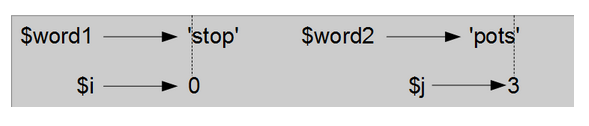
\includegraphics[scale=0.5]{figs/state6.png}}
\caption{State diagram.}
\label{fig.state4}
\end{figure}

We took some license by arranging the variables in the frame
and adding dotted lines to show that the values of {\tt \$i} 
and {\tt \$j} indicate characters in {\tt \$word1} and 
{\tt \$word2}.

Starting with this diagram, run the program on paper, changing 
the values of {\tt \$i} and {\tt \$j} during each iteration. 
Find and fix the second error in this function. (\emph{Solution:} \ref{sol_isreverse}).
\label{isreverse}
\index{is-reverse}


\section{Glossary}

\begin{description}

\item[object:] Something a variable can refer to.  For now,
you can use ``object'' and ``value'' interchangeably.
\index{object}

\item[sequence:] An ordered collection of
values where each value is identified by an integer index.
\index{sequence}

\item[item:] One of the values in a sequence.
\index{item}

\item[index:] An integer value used to select an item in
a sequence, such as a character in a string.  In Perl
indices start from 0.
\index{index}

\item[slice:] A part of a string specified by a range of indices.
\index{slice}

\item[empty string:] A string with no characters and length 0, represented
by two quotation marks.
\index{empty string}

\item[immutable:] The property of a sequence whose items cannot
be changed.
\index{immutability}

\item[traverse:] To iterate through the items in a sequence,
performing a similar operation on each.
\index{traversal}

\index{search}
\item[search:] A pattern of traversal that stops
when it finds what it is looking for.
\index{search!pattern}
\index{pattern!search}

\index{counter}
\item[counter:] A variable used to count something, usually initialized
to zero and then incremented.

\index{regular expression}
\item[regular expressions:] A computing sub-language derived 
from the formal language theory.

\index{pattern}
\item[pattern:] A sequence of characters using a special 
syntax to describe from left to right the content that 
is intended to be matched within a target string.

\index{regex}
\item[regexes:] A pattern-matching sub-language of Perl~6 
derived from the regular expressions.

\index{backtracking}
\item[backtracking:] the process by which when a given attempt 
to match a string fails, the regex engine abandons part of 
the current match attempt, goes back into the string and 
tries to see if it can find another route to a successful 
match. The backtracking process eventually stops as soon 
as a successful match succeeds, or ultimately when all 
possible match possibilities have failed.

\end{description}


\section{Exercises}


\begin{exercise}
\label{count_a}
\index{count method}
\index{method!count}

Write a subroutine that uses the {\tt index} function in a 
loop to count the number of ``a'' in \verb"'banana'",
as we did in the \ref{counter} section. Modify it to count 
any letter in any word passed as arguments to the subroutine.

Write another subroutine counting a given letter in a given 
word and using the {\tt substr} function.

Solutions: \ref{sol_count_a}
\end{exercise}


\begin{exercise}

\label{islower}
\index{lower case!character class}
The \verb'<[a..z]>' character class matches any lower case 
character (only plain ASCII lower case characters, not 
Unicode characters). The following subroutine:

\begin{verbatim}[fontshape=up]
sub is-lower (Str $char) { 
    return so $char ~~ /^<[a..z]>$/
}
\end{verbatim}

should return {\tt True} if its argument is an ASCII lower case 
letter and False otherwise. Test that it works as 
expected (and amend it if needed). The {\tt so} function 
coerces the result of the regex match into a boolean value.

The following subroutines use the {\tt is-lower} subroutine 
and are all supposedly {\em intended} to check 
whether a string contains any lowercase letters, but at 
least some of them are wrong.  Analyze each subroutine by hand, 
determine whether it is correct and describe what it 
actually does (assuming that the parameter is a string). Then 
test them with various input strings to check whether your 
analysis was correct.

\begin{verbatim}[fontshape=up]
sub any_lowercase1(Str $string){
    for $string.comb -> $char {
        if is-lower $char {
            return True;
        } else {
            return False;
        }
    }
}

sub any_lowercase2(Str $string){
    for $string.comb -> $char {
        if is-lower "char" {
            return True;
        } else {
            return False;
        }
    }
}

sub any_lowercase3(Str $string){
    my $flag;
    for $string.comb -> $char {
        $flag =  is-lower $char;
    }
    return $flag;
}

sub any_lowercase4(Str $string){
    my $flag = False;
    for $string.comb -> $char {
        $flag = $flag or is-lower $char;
    }
    return $flag;
}

sub any_lowercase5(Str $string){
    my $flag = False;
    for $string.comb -> $char {
        if is-lower $char {
            $flag = True;
        }
    }
    return $flag;
}

sub any_lowercase6(Str $string){
    for $string.comb -> $char {
        if is-lower $char {
            return 'True';
        }
    }
    return 'False';
}

sub any_lowercase7(Str $string){
    for $string.comb -> $char {
        return True if is-lower $char;
    }
    return False;
}

sub any_lowercase8(Str $string){
    for $string.comb -> $char {
        return False unless is-lower $char;
    }
    return True;
}

sub any_lowercase9(Str $string){
    for $string.comb -> $char {
        if not is-lower $char {
            return False;
        }
    return True;
    }
}
\end{verbatim}

Solution: \ref{sol_islower}.

\end{exercise}


\begin{exercise}
\index{letter rotation}
\index{rotation, letter}
\index{Caesar cipher}

\label{rotate}
A Caesar cipher is a weak form of encryption that involves ``rotating'' each
letter by a fixed number of places.  To rotate a letter means
to shift it through the alphabet, wrapping around to the beginning if
necessary, so 'A' rotated by 3 is 'D' and 'Z' rotated by 1 is 'A'.

To rotate a word, rotate each letter by the same amount.
For example, ``cheer'' rotated by 7 is ``jolly'' and ``melon'' rotated
by -10 is ``cubed''.  In the movie {\em 2001: A Space Odyssey}, the 
ship computer is called HAL, which is IBM rotated by -1.

Write a function called \verb"rotate-word"
that takes a string and an integer as parameters, and returns
a new string that contains the letters from the original string
rotated by the given amount.  

You might want to use the built-in functions {\tt ord}, which 
converts a character to a numeric code, and {\tt chr}, which 
converts numeric codes back to characters.  
\begin{verbatim}[fontshape=up]
> say 'c'.ord;
99
> say chr 99
c
\end{verbatim}
%

Letters of the alphabet are encoded in alphabetical
order, so for example:

\begin{verbatim}[fontshape=up]
> ord('c') - ord('a')
2
\end{verbatim}

Because \verb"'c'" is the two-eth letter of the alphabet.  But
beware: the numeric codes for upper case letters are different.

\index{rot13}
Potentially offensive jokes on the Internet are sometimes 
encoded in ROT13, which is a Caesar cipher with rotation 13. 
Since 13 is the half the number of letters in our alphabet, 
applying rotation 13 twice gives back the original word, 
so that the same procedure can be used for both encoding 
and decoding in rotation 13. If you are not
easily offended, find and decode some of these jokes.  Solution: \ref{sol_rotate}.

\end{exercise}

